% Manuscript draft - Journal of Chemical & Engineering Data (ACS), two-column achemso layout.
% Compile with:  latexmk -pdf main.tex   (or upload manuscript/ and figures/ to Overleaf; set the main file to main.tex)
% Remaining TODO: author names, e-mail, acknowledgement. References marked VERIFY in references.bib.
\documentclass[journal=jceaax,manuscript=article,layout=twocolumn]{achemso}

\usepackage[version=4]{mhchem}
\usepackage{amsmath}
\usepackage{graphicx}
\usepackage{booktabs}
\usepackage{siunitx}
\usepackage{url}
\graphicspath{{../figures/}}

\author{Member One}       % TODO: replace with the group members' names
\author{Member Two}
\author{Member Three}
\author{Member Four}
\author{Member Five}
\affiliation{Department of Chemical Engineering, Indian Institute of Technology Gandhinagar, Palaj, Gandhinagar 382355, Gujarat, India}
\email{student@iitgn.ac.in}  % TODO: corresponding author

\title{A Rule-Based Engine for the Apparent Specific Heat of Multiphase Fluids from Arbitrary Combinations of Thermodynamic Data}

\abstract{
We present an open-source engine that computes the isobaric heat capacity of single- and multiphase
fluids (solutions, suspensions, emulsions and slurries with phase change) from \emph{any} consistent
subset of thermodynamic information: temperature, pressure, composition in any representation,
heat, work, $\Delta H$, $\Delta U$, $\Delta S$, $C_V$ or $\gamma$. Twenty-five thermodynamic relations are
encoded as rules and evaluated by forward chaining. All routes allowed by the input are computed
and compared, inconsistent over-specification is detected, and missing information is identified.
The property route combines pure-component correlations, NRTL excess heat capacities obtained
through the Gibbs--Helmholtz equation, mass-weighted phase averaging and latent contributions from
melting, solid--liquid equilibrium and dissolution. Validation uses only published data:
521 data points from NIST SRD~69, the NIST ThermoML archive, nanofluid calorimetry and freezing-point tables.
Pure-liquid heat capacities agree with NIST to 0.33\,\% (AARD). NRTL parameters regressed from
vapor--liquid equilibria underpredict the excess heat capacity of water + alcohols six-fold or more; refitting them to excess enthalpies at several temperatures reduces the excess-enthalpy
error from 256 to \SI{28}{J.mol^{-1}} (ethanol) and the heat-capacity error of water + methanol
from 6.5\,\% to 2.7\,\% on independent data. For 69 nanofluid points the thermal-equilibrium (mass-weighted)
model gives 2.1\,\% AARD, against 18.5\,\% for the volume-weighted model. Freezing points of aqueous
ethanol in the ice-slurry range are reproduced to \SI{0.84}{K}.
}

\begin{document}

\section{Introduction}
The isobaric specific heat $c_p$ of process fluids enters every energy balance, yet many industrially
relevant fluids are not single phases. Nanofluids and catalyst slurries are suspensions, cutting fluids
and foods are emulsions, and ice slurries and phase-change-material (PCM) slurries partly melt within
their working range. Three questions must be answered before a value of $c_p$ can be quoted for such a
fluid: (i) which mixing rule is thermodynamically correct for the phases present; (ii) how large the
excess contribution of each liquid solution is; and (iii) how much latent heat is absorbed as the phase
amounts change with temperature.

A second difficulty is that the available information differs from case to case. An experimentalist
may know the heat supplied and the temperature rise, a designer the composition and temperature, and a
table may provide $\Delta S$ or $C_V$. Most tools implement one route and fail when its inputs are missing.
This work builds a \emph{general} engine. The user provides whatever is known; thermodynamic relations,
represented as explicit rules, are chained until $c_p$ is obtained; and the derivation is reported step
by step.

\section{Theory and Methodology}
\subsection{Relation network and forward chaining}
Each relation is a rule $\{\text{inputs}\}\rightarrow\{\text{outputs}\}$. A knowledge base is
initialised with the user inputs converted to SI units, and any rule whose inputs are all known is
applied until no rule fires. Consistency rules (e.g.\ $\Delta H = Q + W$ at constant $P$) are also
evaluated when their output is already known, and a warning is issued if the two values differ by more
than 2\,\%. If no heat-capacity candidate is produced, a backward search over the rule graph returns
the smallest sets of additional inputs that would complete a route.

\subsection{Route A: property route}
Pure-component heat capacities use DIPPR equations 100 and 107 \cite{Perry2008}, NIST Shomate equations
for solids \cite{NISTWebBook} and the IAPWS-06 equation of state for ice \cite{Feistel2006,IAPWS2009}.
Enthalpies follow from Kirchhoff's law along a path through the melting and boiling points.

For an ideal liquid mixture $C_p=\sum_i x_iC_{p,i}$. For a real solution the excess heat capacity
follows from the NRTL model \cite{Renon1968} through the Gibbs--Helmholtz equation,
\begin{equation}
H^E=-RT^2\left(\frac{\partial (G^E/RT)}{\partial T}\right)_{P,x},\qquad
C_p^E=\left(\frac{\partial H^E}{\partial T}\right)_{P,x},
\end{equation}
with $\tau_{ij}=a_{ij}+b_{ij}/T+e_{ij}\ln T$. The derivatives are evaluated by central differences with
step $h=10^{-4}T$, which balances $O(h^2)$ truncation against $O(\epsilon/h^2)$ round-off. They agree with
exact symbolic derivatives to $10^{-4}$.

Because $C_p^E$ is a second temperature derivative of $G^E/RT$, parameters regressed from VLE data are
not expected to reproduce it. We therefore refitted the water + ethanol and water + methanol parameters
to measured excess enthalpies at 298--383~K \cite{Nagamachi2006,Brandt2014,Modaresifar2017,Dettmann2006,Behbehani2006}
taken from the NIST ThermoML archive \cite{ThermoMLArchive}. Candidate parameter sets
($\alpha = 0.2$--0.47, with and without $e_{ij}$) were accepted only if $\Delta G_\mathrm{mix}/RT$ remained convex
in composition between 240 and 390~K, i.e.\ if the model predicted no spurious liquid--liquid split.

In a heterogeneous mixture enthalpy is additive over phases, so $c_p=\sum_p w_p c_{p,p}$ with mass
fractions $w_p$. For a nanofluid with particle volume fraction $\phi$ this is identical to the
thermal-equilibrium model (Model II) \cite{Xuan2000},
\begin{equation}
c_p=\frac{\phi\rho_s c_{p,s}+(1-\phi)\rho_f c_{p,f}}{\phi\rho_s+(1-\phi)\rho_f},
\end{equation}
whereas the volume-weighted Model I, $c_p=\phi c_{p,s}+(1-\phi)c_{p,f}$ \cite{Pak1998}, weights a quantity
defined per unit mass by a volume fraction and is inconsistent unless $\rho_s=\rho_f$.

\subsection{Phase change and apparent heat capacity}
The total enthalpy is $H(T)=\sum_p\sum_i n_i^pH_i^p(T)+\sum_{p\in L}n^pH^{E,p}(T,\mathbf{x}^p)$. The phase
amounts $n_i^p(T)$ follow from (a) a smoothed melting step
$f(T)=\tfrac12[1+\mathrm{erf}((T-T_m)/\sigma\sqrt2)]$ for pure dispersed components; (b) solid--liquid
equilibrium for components crystallising from a solution,
\begin{equation}
\ln(x_k\gamma_k)=-\frac{\Delta H_\mathrm{fus}}{R}\left(\frac1T-\frac1{T_m}\right)
+\frac{\Delta C_p}{R}\left(\frac{T_m}{T}-1-\ln\frac{T_m}{T}\right),
\end{equation}
where the $\Delta C_p$ term keeps the equilibrium consistent with the Kirchhoff enthalpies; or (c) tabulated
solubility for electrolytes. The chain rule then splits the apparent heat capacity into three parts,
\begin{equation}
c_{p,\mathrm{app}}=\frac{dH}{dT}=\underbrace{\sum n_i^pC_{p,i}^p}_{\text{ideal}}
+\underbrace{\sum n^pC_p^{E,p}}_{\text{excess}}
+\underbrace{\sum \frac{\partial H}{\partial n_i^p}\frac{dn_i^p}{dT}}_{\text{latent}},
\end{equation}
and the interval mean is $[H(T_2)-H(T_1)]/[m(T_2-T_1)]$.

\subsection{Routes B and C}
With $Q>0$ for heat added and $W>0$ for work done on the system, the first law gives $\Delta H = Q + W$ at
constant pressure ($W$ = shaft work) and $\Delta U = Q + W$ at constant volume, so
$c_p=\Delta H/(m\Delta T)$ and $c_V=\Delta U/(m\Delta T)$. Further routes use $c_p=\Delta S/[m\ln(T_2/T_1)]$ (constant
$P$ and $c_p$), $c_p=\gamma c_V$ and the exact identity $c_p=c_V+Tv\alpha^2/\kappa_T$ \cite{Smith2018}.

\section{Computational Details}
The engine is written in Python (NumPy, SciPy, pandas, Matplotlib). It contains 13 components and binary
data in JSON files, each value with its source; adding a component requires no code change. Validation
data were obtained as follows:
\begin{itemize}
\item downloaded from NIST SRD~69 \cite{NISTFluid};
\item extracted from the NIST ThermoML archive \cite{ThermoMLArchive}: 876 binary points, each traced to its original paper;
\item digitised from the vector figures of an open-access calorimetry study \cite{OHanley2012}, reading marker coordinates from the PDF drawing commands;
\item taken from a handbook table of freezing points \cite{Lange1967}.
\end{itemize}
The software passes 127 automated tests, including regression tests against these data.

\section{Results and Discussion}
Table~\ref{tab:aard} summarises the validation.

\subsection{Pure components}
Over 128 NIST SRD~69 points for five liquids the AARD is 0.33\,\% (Figure~\ref{fig:pure} shows toluene,
the worst case). The $C_V\rightarrow C_p$ route applied to NIST $c_V$ of water reproduces NIST $c_p$ to 0.12\,\%.

\begin{figure}
  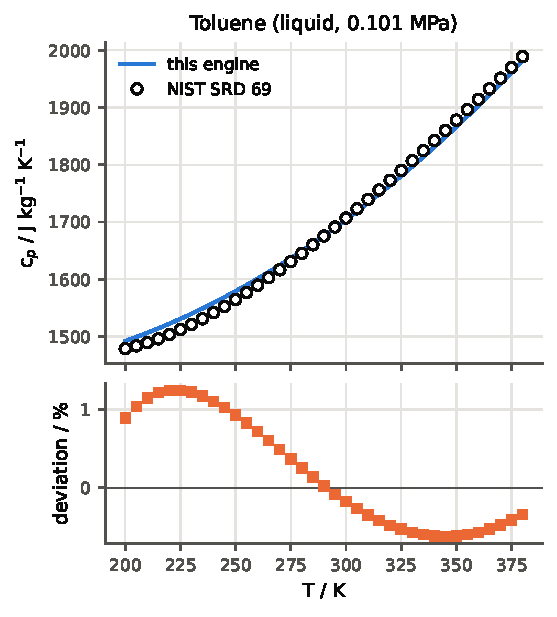
\includegraphics[width=\columnwidth]{val1_toluene}
  \caption{Liquid heat capacity of toluene at 0.101~MPa: DIPPR equation 100 vs NIST SRD~69.}
  \label{fig:pure}
\end{figure}

\subsection{Real solutions: excess enthalpy and excess heat capacity}
With VLE-regressed NRTL parameters the excess enthalpy of water + ethanol is poorly described
(RMSD \SI{256}{J.mol^{-1}}; Figure~\ref{fig:he}). In particular, the change of sign of $H^E$ between 298 and
363~K is missed. The refitted parameters reduce the RMSD to \SI{28}{J.mol^{-1}}; for water + methanol the
reduction is from 141 to \SI{23}{J.mol^{-1}}. Because two isotherms (298.15 and 323.15~K) were measured with
the same apparatus \cite{Nagamachi2006}, their finite difference gives a model-free estimate of the mean
$C_p^E$ of water + ethanol over that interval. This estimate peaks at \SI{14.5}{J.mol^{-1}.K^{-1}} near
$x_\mathrm{EtOH}=0.2$ (Figure~\ref{fig:cpe}). The refitted model reproduces it with an RMSD of
\SI{2.3}{J.mol^{-1}.K^{-1}}, whereas the VLE parameters give a peak of only about \SI{2}{J.mol^{-1}.K^{-1}}.

The decisive test uses heat capacities that were \emph{not} used in any fit. For water + methanol at 280
and 320~K and 0.1~MPa \cite{Tanaka2007}, the ideal-mixture rule gives 7.5\,\% AARD, the VLE-NRTL model 6.5\,\%
and the $H^E$-refitted model 2.7\,\% (Figure~\ref{fig:meoh}). The largest remaining deviations occur at
280~K, below the range of the excess-enthalpy data. For ethanol + toluene, for which no binary parameters
are available, the ideal fallback underestimates $C_p$ by 8.3\,\% \cite{VegaMaza2011}. This shows the
importance of binary caloric data; the engine warns whenever it falls back to ideal mixing.

\begin{figure}
  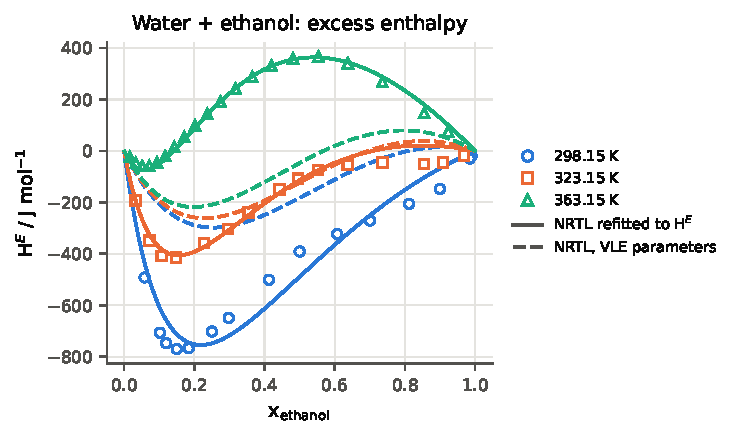
\includegraphics[width=\columnwidth]{fig_HE_water_ethanol}
  \caption{Excess enthalpy of water + ethanol: data \cite{Nagamachi2006,Brandt2014} and NRTL with VLE-fitted and $H^E$-refitted parameters.}
  \label{fig:he}
\end{figure}

\begin{figure}
  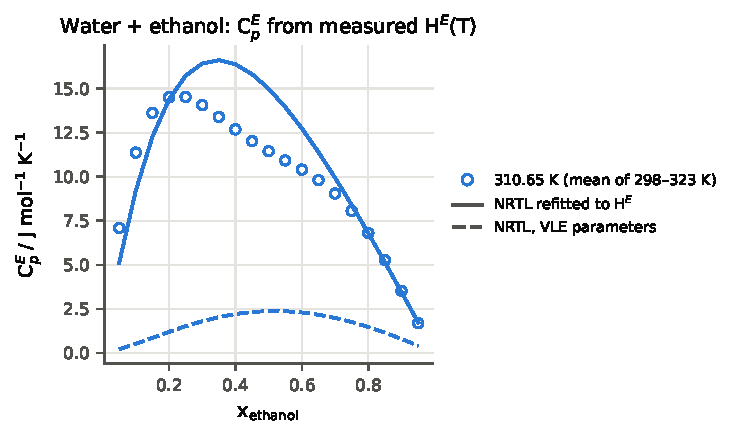
\includegraphics[width=\columnwidth]{fig_cpE_from_HE_water_ethanol}
  \caption{Mean excess heat capacity of water + ethanol between 298.15 and 323.15~K obtained from measured $H^E$ \cite{Nagamachi2006}, compared with NRTL.}
  \label{fig:cpe}
\end{figure}

\begin{figure}
  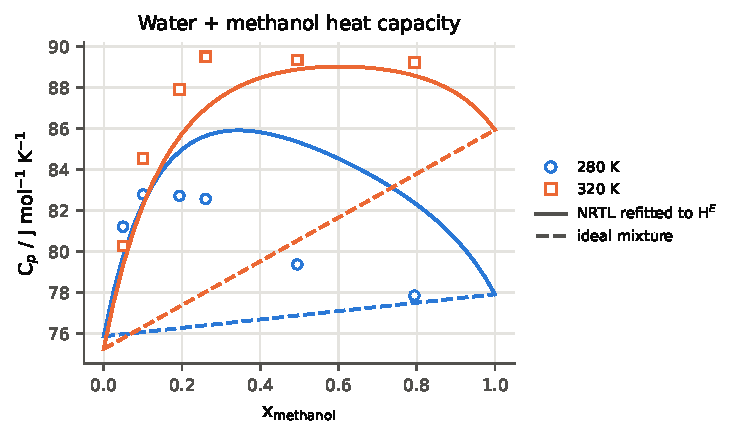
\includegraphics[width=\columnwidth]{fig_cp_methanol_water}
  \caption{Heat capacity of water + methanol at 0.1~MPa \cite{Tanaka2007}: ideal mixture and NRTL with $H^E$-refitted parameters (independent prediction).}
  \label{fig:meoh}
\end{figure}

\subsection{Nanofluids}
For 69 DSC measurements on \ce{Al2O3}, \ce{CuO} and \ce{SiO2} in water at 35--55~$^\circ$C \cite{OHanley2012},
Model~II, which the engine evaluates directly as the mass-weighted Route~A, gives an AARD of 2.1\,\%
(maximum 5.3\,\%). Model~I gives 18.5\,\% (maximum 63\,\% for CuO, whose density is six times that of water;
Figure~\ref{fig:nano}). These results agree with the conclusions of the original authors and of
\citet{Zhou2008}, and confirm that mixing rules must use mass fractions.

\begin{figure}
  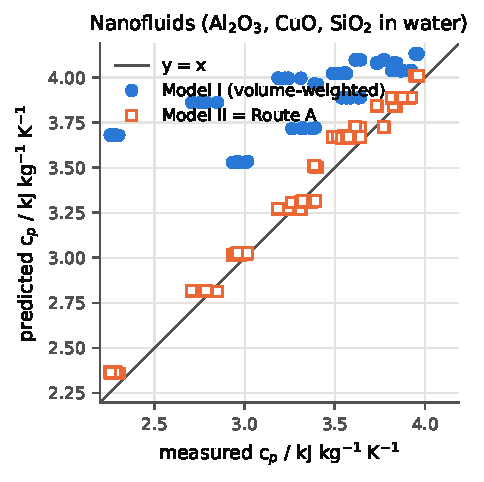
\includegraphics[width=\columnwidth]{fig_nanofluid_parity}
  \caption{Predicted vs measured specific heat of water-based nanofluids \cite{OHanley2012}.}
  \label{fig:nano}
\end{figure}

\subsection{Slurries with phase change}
The latent part of the apparent heat capacity of an ice slurry is governed by the liquidus. For 13
freezing points of aqueous ethanol up to 30~wt\,\% \cite{Lange1967}, the ideal equation with the $\Delta C_p$
correction gives a mean deviation of 0.84~K (1.06~K without it; Figure~\ref{fig:freeze}). NRTL activity
coefficients, extrapolated from 298--383~K, make the prediction worse (2.1--3.3~K), so the ideal form is
the default. Above 40~wt\,\% the liquid is deeply supercooled and all models deviate by several kelvin.
For a 10~wt\,\% ethanol ice slurry the apparent heat capacity rises to about 70~kJ\,kg$^{-1}$\,K$^{-1}$ just below
the liquidus and falls to the solution value above it (Figure~\ref{fig:ice}). The integral of the apparent
heat capacity over a melting peak equals the enthalpy change to $10^{-8}$\,\% for a PCM slurry.

\begin{figure}
  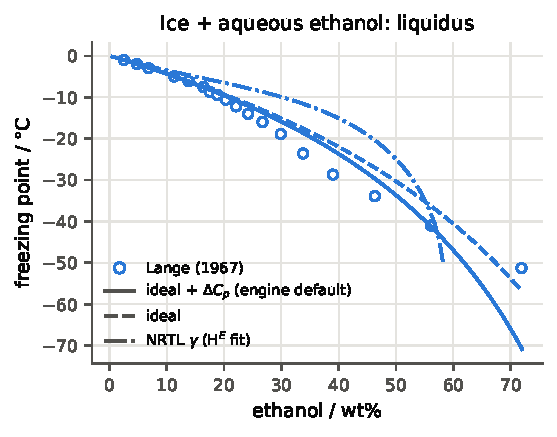
\includegraphics[width=\columnwidth]{fig_freezing_points}
  \caption{Freezing points of water + ethanol \cite{Lange1967} and predictions of the solid--liquid-equilibrium models.}
  \label{fig:freeze}
\end{figure}

\begin{figure}
  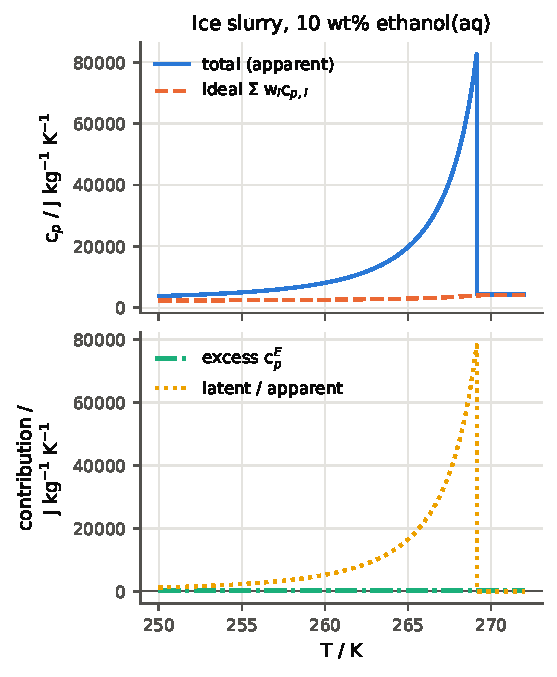
\includegraphics[width=\columnwidth]{fig_cpT_ice_ethanol_10wt}
  \caption{Apparent heat capacity of an ice slurry in 10~wt\,\% aqueous ethanol and its ideal, excess and latent contributions.}
  \label{fig:ice}
\end{figure}

\subsection{Consistency between routes}
For seven systems, from pure water to a five-component emulsion with suspended silica and two
phase-change slurries, the enthalpy change predicted by Route~A was fed back to Route~B as a measured
heat. The recovered heat capacities agree to better than $10^{-6}$\,\%.

\begin{table*}
  \caption{Validation summary (generated by \texttt{validation/run\_all.py}; full table in the Supporting Information).}
  \label{tab:aard}
  \small
  \begin{tabular}{c p{8.6cm} c r r r}
\toprule
Case & Comparison & Metric & $N$ & mean & max \\
\midrule
1 & 5 pure liquids vs NIST SRD 69 (0.1 MPa) & AARD \% & 128 & 0.33 & 1.25 \\
1 & 4 compounds, literature point values & AARD \% & 15 & 0.716 & 2.37 \\
1 & water: cp from NIST cv, cp = cv + Tv$\alpha^2$/$\kappa_T$ & AARD \% & 20 & 0.125 & 0.762 \\
2 & ethanol + water: H$^E$, NRTL (VLE parameters) & RMSD J/mol & 88 & 256 & 630 \\
2 & ethanol + water: H$^E$, NRTL (refitted to H$^E$) & RMSD J/mol & 88 & 28.4 & 104 \\
2 & methanol + water: H$^E$, NRTL (VLE parameters) & RMSD J/mol & 151 & 141 & 344 \\
2 & methanol + water: H$^E$, NRTL (refitted to H$^E$) & RMSD J/mol & 151 & 23.2 & 98.1 \\
2 & methanol + water: Cp, ideal mixture & AARD \% & 12 & 7.47 & 12.8 \\
2 & methanol + water: Cp, NRTL, VLE parameters & AARD \% & 12 & 6.51 & 11.4 \\
2 & methanol + water: Cp, NRTL refitted to H$^E$ & AARD \% & 12 & 2.71 & 7.54 \\
2 & ethanol + toluene: Cp, ideal fallback (no NRTL parameters) & AARD \% & 11 & 8.33 & 12.3 \\
2 & glycerol + water: H$^E$, ideal fallback (H$^E$ = 0) & RMSD J/mol & 9 & 466 & 611 \\
2 & ethanol + water: mean Cp$^E$ 298-323 K from measured H$^E$(T), NRTL, VLE parameters & RMSD J/(mol K) & 19 & 9.12 & 13.3 \\
2 & ethanol + water: mean Cp$^E$ 298-323 K from measured H$^E$(T), NRTL refitted to H$^E$ & RMSD J/(mol K) & 19 & 2.31 & 4.1 \\
3 & all nanofluids: cp, Model I & AARD \% & 69 & 18.5 & 63.3 \\
3 & all nanofluids: cp, Model II = Route A & AARD \% & 69 & 2.06 & 5.28 \\
4 & ice + water + ethanol: freezing point, ideal, $\le$ 30 wt\% (ice-slurry range) & $|\Delta T|$ K & 13 & 1.06 & 3.85 \\
4 & ice + water + ethanol: freezing point, ideal + $\Delta C_p$ (engine default), $\le$ 30 wt\% (ice-slurry range) & $|\Delta T|$ K & 13 & 0.842 & 3.08 \\
4 & ice + water + ethanol: freezing point, NRTL $\gamma$ (H$^E$ fit), $\le$ 30 wt\% (ice-slurry range) & $|\Delta T|$ K & 13 & 3.31 & 9 \\
4 & ice + water + ethanol: freezing point, NRTL $\gamma$ (VLE fit), $\le$ 30 wt\% (ice-slurry range) & $|\Delta T|$ K & 13 & 2.06 & 6.57 \\
4 & ice + water + ethanol: engine liquidus vs SLE equation & $|\Delta T|$ K & 13 & 1.5e-08 & 1.5e-08 \\
4 & ice ethanol 10wt: $\int$cp app dT vs $\Delta H$ (energy conservation) & rel. dev \% & 1601 & 0.109 & 0.109 \\
4 & pcm octadecane 20wt: $\int$cp app dT vs $\Delta H$ (energy conservation) & rel. dev \% & 1601 & 7.8e-09 & 7.8e-09 \\
5 & Route B vs Route A, 7 systems & rel. dev \% & 7 & 1.9e-07 & 6.2e-07 \\
\bottomrule
\end{tabular}

\end{table*}

\section{Conclusions}
A rule-based engine computes the heat capacity of multiphase fluids from any consistent combination of
thermodynamic information. It reports the derivation, compares independent routes and identifies
missing information. Validation against 521 published data points supports four
conclusions:
\begin{enumerate}
\item Pure-component and Cp--Cv relations are accurate to better than 0.5\,\%.
\item The excess heat capacity of aqueous alcohols requires NRTL parameters fitted to excess enthalpies at several temperatures. VLE parameters underpredict it six-fold or more. With $H^E$-fitted parameters the heat capacity of water + methanol is predicted to 2.7\,\% from independent data.
\item Mixing rules for suspensions must use mass fractions: the volume-weighted rule errs by up to 63\,\%.
\item The latent contribution of ice slurries follows from solid--liquid equilibrium, reproduced to better than 1~K in the useful concentration range.
\end{enumerate}
Remaining limitations are the need for binary caloric data, the absence of vapour--liquid equilibrium
for mixtures and of solute partitioning in emulsions, and approximate electrolyte thermodynamics.

\begin{acknowledgement}
TODO: course instructor and teaching assistants of CL~202, IIT Gandhinagar.
\end{acknowledgement}

\begin{suppinfo}
Full validation table, rule list, component database with sources, data-extraction scripts, test suite and the demonstration notebook.
\end{suppinfo}

\bibliography{references}

\end{document}
